% Common preamble for PIGMIE patent figures (A4).
% Drawing conventions:
%   - A4 portrait
%   - Sans-serif throughout (Helvetica)
%   - "Fig. N" sentence-case caption near top
%   - Page "N/total" at top centre
%   - Reference numerals outside boxes via leader lines
%   - ALL CAPS labels in component boxes
%   - Reactor uses north-east-lines hatched fill
%   - Scene uses double-line border
%   - Module enclosures use dashed line with internal numeral

\documentclass[a4paper,10pt]{article}
\usepackage[top=2.5cm,bottom=1.0cm,left=2.5cm,right=1.5cm]{geometry}
\usepackage[T1]{fontenc}
\usepackage{helvet}
\renewcommand{\familydefault}{\sfdefault}
\usepackage{amsmath,amssymb,bm}
\usepackage{tikz}
\usetikzlibrary{shapes,shapes.geometric,shapes.misc,arrows.meta,positioning,fit,calc,backgrounds,decorations.pathreplacing,decorations.markings,patterns}
\pagestyle{empty}
\setlength{\parindent}{0pt}

\tikzset{
  % Component box: ALL CAPS label inside, no numeral inside
  cbox/.style={draw, rectangle, minimum height=1.0cm, minimum width=2.4cm,
               align=center, line width=0.5pt, font=\small},
  cbox-tall/.style={cbox, minimum height=1.6cm},
  cbox-wide/.style={cbox, minimum width=3.0cm},
  cbox-narrow/.style={cbox, minimum width=1.8cm, font=\footnotesize},
  % Reactor / physical medium: hatched fill
  reactor/.style={cbox, pattern=north east lines, pattern color=black!70},
  % Scene: double-line border
  scenebox/.style={cbox, double, double distance=1.2pt, line width=0.4pt},
  % Module / sub-module enclosure
  enclosure/.style={draw, rectangle, dashed, line width=0.4pt, inner sep=10pt, rounded corners=2pt},
  enclosure-solid/.style={draw, rectangle, line width=0.5pt, inner sep=10pt, rounded corners=2pt},
  % Arrows
  flowarr/.style={-Latex, line width=0.5pt, font=\scriptsize},
  flowbi/.style={Latex-Latex, line width=0.5pt, font=\scriptsize},
  flowarr-fb/.style={-Latex, line width=0.5pt, dashed, font=\scriptsize},
  % Reference numeral leader-line endpoint and label
  refnum/.style={font=\footnotesize, inner sep=1pt},
  leader/.style={line width=0.4pt, -Latex},
  % Caption banner
  figcap/.style={font=\bfseries\large}
}

% Helper: figure header (page number + Fig. N caption)
\newcommand{\figheader}[3]{%
  % #1 = page number (e.g. "1"), #2 = total pages, #3 = figure label (e.g. "1" or "4A")
  \noindent\hfill\small #1/#2\hfill\null\par
  \vspace{0.2cm}
  \begin{center}\bfseries Fig.\ #3\end{center}
  \vspace{0.2cm}
}


\begin{document}

\figheader{7}{7}{6}

\begin{center}
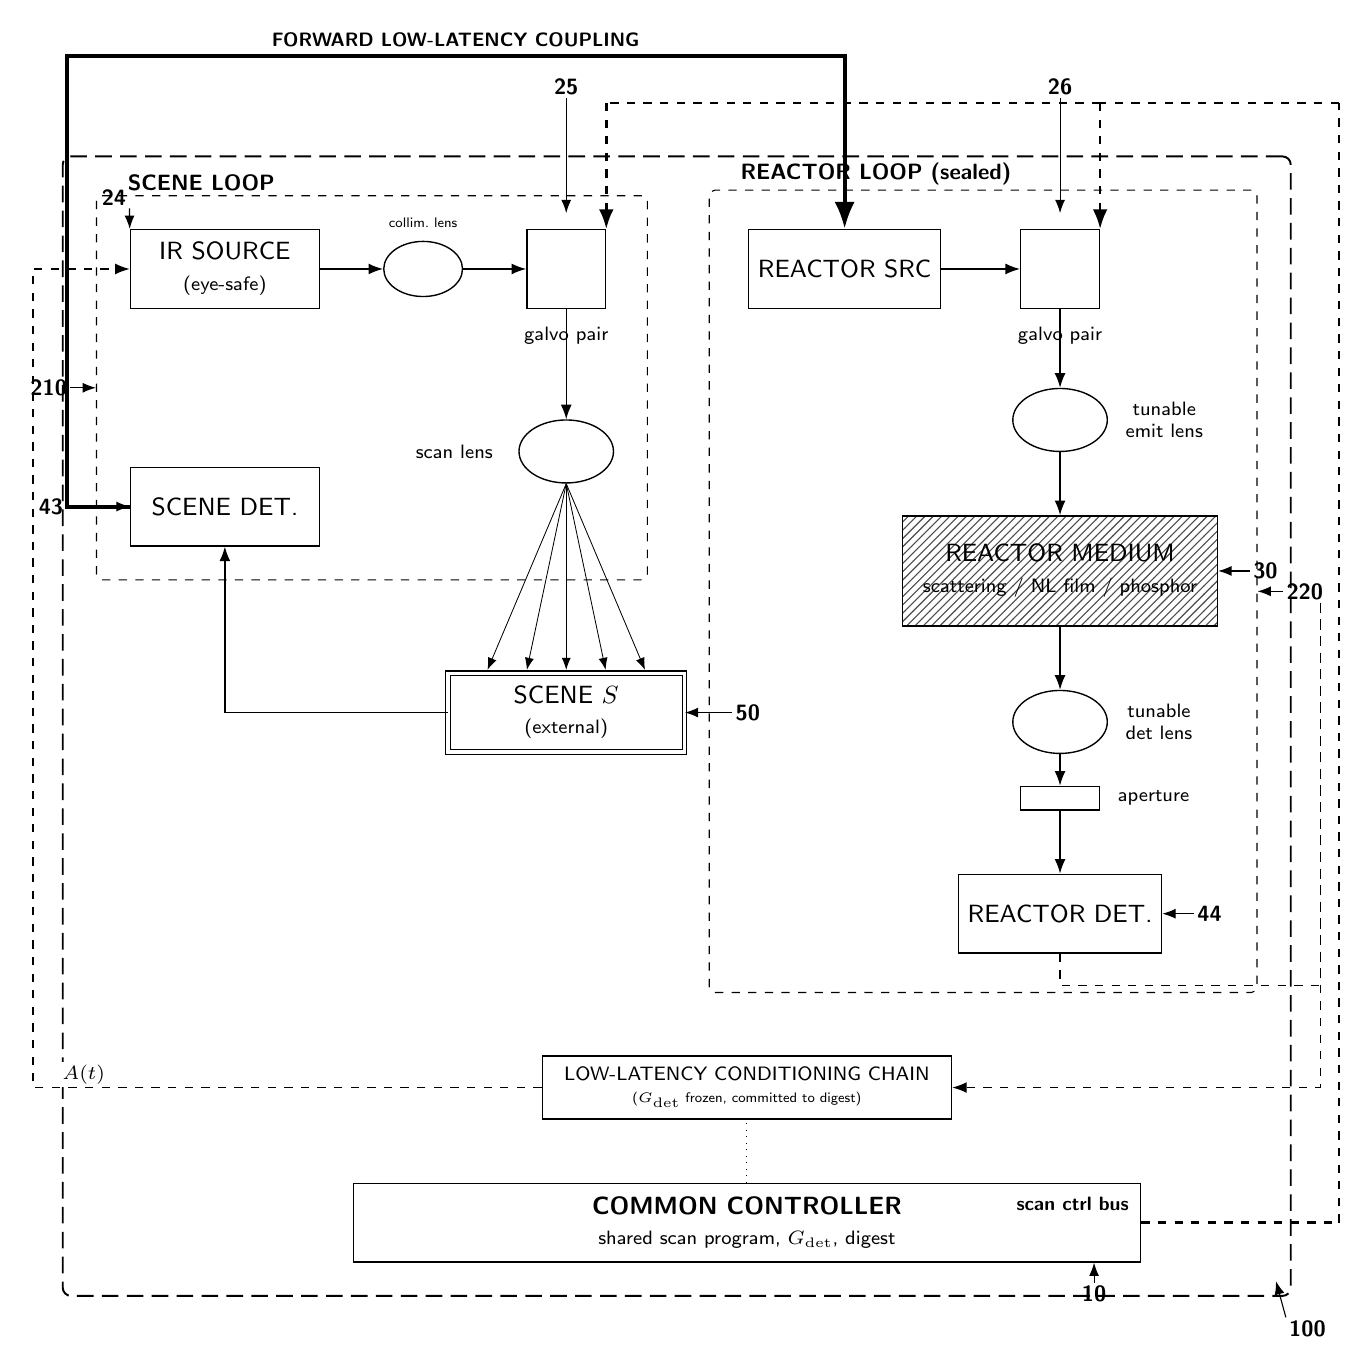
\begin{tikzpicture}[node distance=8mm]

% ============== LEFT PANE: SCENE LOOP (210) — does NOT contain external scene ==============
\node[cbox, minimum width=2.4cm] (irsrc) {IR SOURCE\\\scriptsize (eye-safe)};
\node[draw, ellipse, line width=0.5pt, right=8mm of irsrc, minimum width=10mm, minimum height=7mm] (collim) {};
\node[font=\tiny, above=0.5mm of collim] {collim.\ lens};
\node[draw, line width=0.5pt, right=8mm of collim, minimum width=10mm, minimum height=10mm] (sgalvo) {};
\node[font=\scriptsize, below=1mm of sgalvo] {galvo pair};
\node[draw, ellipse, line width=0.5pt, below=14mm of sgalvo, minimum width=12mm, minimum height=8mm] (slens) {};
\node[font=\scriptsize, left=2mm of slens] {scan lens};
\node[cbox, below=20mm of irsrc, minimum width=2.4cm] (sdet) {SCENE DET.};

\draw[flowarr] (irsrc.east) -- (collim.west);
\draw[flowarr] (collim.east) -- (sgalvo.west);
\draw[flowarr] (sgalvo.south) -- (slens.north);

% Scene loop enclosure: contains source / collim / galvo / scan lens / scene detector ONLY
% Scene S itself is EXTERNAL and sits below this enclosure
\begin{scope}[on background layer]
  \node[enclosure, fit=(irsrc)(collim)(sgalvo)(slens)(sdet), inner sep=12pt] (sceneloop) {};
\end{scope}
\node[font=\footnotesize\bfseries, anchor=south west] at ($(sceneloop.north west)+(8pt,-2pt)$)
  {SCENE LOOP};

% External scene S offset below the scene-loop boundary; offset chosen for a clear visual gap
\node[scenebox, below=24mm of slens, minimum width=3.0cm, minimum height=1.0cm] (scene)
  {SCENE $S$\\\scriptsize (external)};

% Scan rays: from slens.south DOWN, terminating on scene.north (explicit endpoints)
\foreach \xoff in {-10mm,-5mm,0mm,5mm,10mm} {
  \draw[-Latex, line width=0.3pt] (slens.south) -- ($(scene.north)+(\xoff,1pt)$);
}

% Scene -> SCENE DET (returning observation; horizontal arrow back to detector)
\draw[flowarr] (scene.west) -| (sdet.south);

% ============== RIGHT PANE: REACTOR LOOP (220) ==============
\node[cbox, right=18mm of sgalvo, minimum width=2.4cm] (rsrc) {REACTOR SRC};
\node[draw, line width=0.5pt, right=10mm of rsrc, minimum width=10mm, minimum height=10mm] (rgalvo) {};
\node[font=\scriptsize, below=1mm of rgalvo] {galvo pair};
\node[draw, ellipse, line width=0.5pt, below=10mm of rgalvo, minimum width=12mm, minimum height=8mm] (relens) {};
\node[font=\scriptsize, right=1mm of relens, align=center] {tunable\\emit lens};

\node[reactor, below=8mm of relens, minimum width=4.0cm, minimum height=1.4cm] (medium)
  {REACTOR MEDIUM\\\scriptsize scattering / NL film / phosphor};

\node[draw, ellipse, line width=0.5pt, below=8mm of medium, minimum width=12mm, minimum height=8mm] (rdlens) {};
\node[font=\scriptsize, right=1mm of rdlens, align=center] {tunable\\det lens};
\node[draw, line width=0.5pt, below=4mm of rdlens, minimum width=10mm, minimum height=3mm] (apert) {};
\node[font=\scriptsize, right=1mm of apert] {aperture};
\node[cbox, below=8mm of apert, minimum width=2.4cm] (rdet) {REACTOR DET.};

\draw[flowarr] (rsrc.east) -- (rgalvo.west);
\draw[flowarr] (rgalvo.south) -- (relens.north);
\draw[flowarr] (relens.south) -- (medium.north);
\draw[flowarr] (medium.south) -- (rdlens.north);
\draw[flowarr] (rdlens.south) -- (apert.north);
\draw[flowarr] (apert.south) -- (rdet.north);

\begin{scope}[on background layer]
  \node[enclosure, fit=(rsrc)(rgalvo)(relens)(medium)(rdlens)(apert)(rdet), inner sep=14pt] (reactorloop) {};
\end{scope}
\node[font=\footnotesize\bfseries, anchor=south west] at ($(reactorloop.north west)+(8pt,-2pt)$)
  {REACTOR LOOP (sealed)};

% ============== CASCADE FORWARD COUPLING (embodiment b) ==============
% Heavy stroke arrow from SCENE DET -> REACTOR SRC. Load-bearing forward
% path of the cascade embodiment: direct (optical via gain-pumped media,
% or electrical), low latency. Distinguishes embodiment (b) from the
% parallel-subsystems variant (a).
% Routed: out of scene loop (west) -> up -> across above both loops ->
% down into rsrc from above. Avoids scene-loop interior elements.
\coordinate (cscOut)  at ($(sdet.west)+(-8mm,0)$);
\coordinate (cscTopR) at ($(rsrc.north)+(0,22mm)$);
\coordinate (cscTopL) at (cscOut |- cscTopR);
\draw[-Latex, line width=1.5pt]
  (sdet.west) -- (cscOut) -- (cscTopL) -- (cscTopR) -- (rsrc.north);
\node[font=\scriptsize\bfseries, align=center, fill=white, inner sep=2pt]
  at ($(cscTopL)!0.5!(cscTopR)+(0,2mm)$)
  {FORWARD LOW-LATENCY COUPLING};

% ============== A(t) feedback path with conditioning chain ==============
% Position chain BELOW reactor loop (chain is body-supported as low-latency path between rdet and irsrc)
\node[draw, line width=0.4pt, font=\scriptsize, align=center, inner sep=4pt,
      minimum width=5.2cm, minimum height=8mm] (gchain) at ($(reactorloop.south)+(-3cm,-12mm)$)
  {LOW-LATENCY CONDITIONING CHAIN\\\tiny ($G_{\mathrm{det}}$ frozen, committed to digest)};

\draw[flowarr-fb] (rdet.south) -- ++(0,-4mm) -| ($(reactorloop.east)+(8mm,0)$) |- (gchain.east);
\draw[flowarr-fb] (gchain.west) -| ($(sceneloop.west)+(-8mm,0)$)
  node[pos=0.45, above, font=\scriptsize\bfseries, fill=white, inner sep=1pt] {$A(t)$}
  |- (irsrc.west);

% ============== COMMON CONTROLLER ==============
\node[cbox-wide, below=8mm of gchain.south, minimum width=10cm, minimum height=1.0cm] (ctrl)
  {\textbf{COMMON CONTROLLER}\\\scriptsize shared scan program, $G_{\mathrm{det}}$, digest};

\draw[line width=0.35pt, dotted] (ctrl.north) -- (gchain.south);

% ============== Module 100 enclosure: visually distinct from inner loops ==============
% Use thicker line + longer dash pattern so module 100 reads as the OUTER boundary
% (matches FIG. 1's dashed module convention)
\begin{scope}[on background layer]
  \node[draw, rectangle, line width=0.7pt, dash pattern=on 6pt off 3pt, rounded corners=3pt,
        inner sep=12pt, fit=(sceneloop)(reactorloop)(gchain)(ctrl)] (mod) {};
\end{scope}

% ============== Shared-scan fan-out: EXTERNAL east bus, drops into NE corners ==============
% Routing constraints:
%   - bus must visibly originate at common controller 10
%   - bus must NOT cross A(t) feedback path
%   - bus branches must NOT be co-located with numeral leaders at galvo.north
%
% Topological analysis: A(t) horizontals at chain.center.y span both
%   left side x ∈ [sceneloop.west - 8mm, chain.west] and right side x ∈ [chain.east, reactorloop.east + 8mm].
% Combined with chain.x range [chain.west, chain.east], the only safe x for an internal bus
% is OUTSIDE module entirely. External east routing satisfies all constraints.
%
% Branches drop into galvo NORTH-EAST corners (not center) so they are clearly separate
% from numeral 25/26 leaders which terminate on galvo north center.

% Bus path waypoints
\coordinate (busExit) at (ctrl.east);
\coordinate (farEastX) at ($(mod.east)+(6mm,0)$);
\coordinate (busOutEast) at (farEastX |- busExit);
\coordinate (busTopY) at ($(sgalvo.north)+(0,16mm)$);
\coordinate (busTopEast) at (farEastX |- busTopY);
\coordinate (busOverRgalvo) at (rgalvo.north east |- busTopY);
\coordinate (busOverSgalvo) at (sgalvo.north east |- busTopY);

% Source label adjacent to bus exit at controller's east edge
\node[font=\scriptsize\bfseries, anchor=south east] at ($(busExit)+(-1pt,1pt)$)
  {scan ctrl bus};

% Bus segments — heavy dashed (0.9pt) for visual prominence
% Path: ctrl.east -> east outside module -> up east outside -> back over module top -> drops into NE corners
\draw[line width=0.9pt, dashed] (busExit) -- (busOutEast);
\draw[line width=0.9pt, dashed] (busOutEast) -- (busTopEast);
\draw[line width=0.9pt, dashed] (busTopEast) -- (busOverRgalvo);
\draw[line width=0.9pt, dashed] (busOverRgalvo) -- (busOverSgalvo);

% Drops with arrowheads into each galvo's NORTH-EAST corner
\draw[line width=0.9pt, dashed, -Latex] (busOverRgalvo) -- (rgalvo.north east);
\draw[line width=0.9pt, dashed, -Latex] (busOverSgalvo) -- (sgalvo.north east);

% ============== Reference numerals ==============
\node[refnum] at ($(sceneloop.west)+(-6mm,0)$) (n210) {\textbf{210}};
\draw[leader] (n210.east) -- (sceneloop.west);
\node[refnum] at ($(reactorloop.east)+(6mm,0)$) (n220) {\textbf{220}};
\draw[leader] (n220.west) -- (reactorloop.east);
\node[refnum] at ($(mod.south east)+(2mm,-4mm)$) (n100) {\textbf{100}};
\draw[leader] (n100.north west) -- ($(mod.south east)+(-2mm,2mm)$);

\node[refnum] at ($(irsrc.north west)+(-2mm,4mm)$) (n24) {\textbf{24}};
\draw[leader] (n24.south east) -- (irsrc.north west);
\node[refnum] at ($(sgalvo.north)+(0,18mm)$) (n25) {\textbf{25}};
\draw[leader] (n25.south) -- ($(sgalvo.north)+(0,2mm)$);
\node[refnum] at ($(rgalvo.north)+(0,18mm)$) (n26) {\textbf{26}};
\draw[leader] (n26.south) -- ($(rgalvo.north)+(0,2mm)$);
\node[refnum] at ($(medium.east)+(6mm,0)$) (n30) {\textbf{30}};
\draw[leader] (n30.west) -- (medium.east);
\node[refnum] at ($(sdet.west)+(-10mm,0)$) (n43) {\textbf{43}};
\draw[leader] (n43.east) -- (sdet.west);
\node[refnum] at ($(rdet.east)+(6mm,0)$) (n44) {\textbf{44}};
\draw[leader] (n44.west) -- (rdet.east);
\node[refnum] at ($(scene.east)+(8mm,0)$) (n50) {\textbf{50}};
\draw[leader] (n50.west) -- (scene.east);
\node[refnum] at ($(ctrl.south east)+(-6mm,-4mm)$) (n10) {\textbf{10}};
\draw[leader] (n10.north) -- ($(ctrl.south east)+(-6mm,0)$);

\end{tikzpicture}
\end{center}

\end{document}
